%This is the Preface
%%=========================================
\addcontentsline{toc}{section}{Abstract}
\begin{center}
\section*{Abstract}
\end{center}

Internet of Things (IoT) applications very often involve the use of sensors. Motion sensing can be used in a vast amount of applications and are therefore very interesting in high volume IoT products. Replacing a battery in such an application is often undesirable, and may in some cases be close to impossible. It is therefore essential for such applications to have sensors that consumes as little power as possible. 

This project thesis presents a thorough analysis of five commercially available microelectromechanical (MEMS), 3-axis accelerometers. The analysis focuses primarily on finding the sensor that gives the best trade-off between functionality and power consumption, with a slightly larger emphasis on the latter. The best sensor is then chosen to be a part of a custom reference board, of which also was designed during this thesis.

The reference board is planned to be used for a Master thesis, where the goal is to further explore different IoT application areas for ultra low power motion sensors.

The project is carried out as feasibility analysis for Disruptive Technologies AS in conjunction with the Norwegian University of Science and Technology (NTNU).

\begin{center}
Trondheim, 2015-12-16\\[1pc]
\begin{figure}[h]
\centering
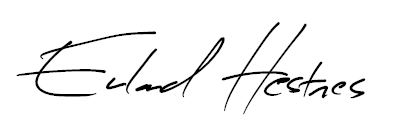
\includegraphics[scale=0.5]{fig/underskrift.png}
\label{fig:underskrift}
\end{figure}
Erlend Hestnes
\end{center}